\documentclass[conference]{IEEEtran}
\IEEEoverridecommandlockouts
% The preceding line is only needed to identify funding in the first footnote. If that is unneeded, please comment it out.
\usepackage{cite}
\usepackage{amsmath,amssymb,amsfonts}
\usepackage{algorithmic}
\usepackage{graphicx}
\usepackage{textcomp}
\usepackage{xcolor}
\def\BibTeX{{\rm B\kern-.05em{\sc i\kern-.025em b}\kern-.08em
    T\kern-.1667em\lower.7ex\hbox{E}\kern-.125emX}}
\begin{document}

\title{CS 846 - Case Study on University of Waterloo's Quest - A Requirement Engineering and User Experience Investigation and Lessons Learned Along the Way\\
{\footnotesize \textsuperscript}
}

\author{\IEEEauthorblockN{Yilun Bai}
\IEEEauthorblockA{\textit{David Cheriton School of Computer Science} \\
\textit{University of Waterloo}\\
Waterloo, Canada \\
yilun.bai@uwaterloo.ca}

}

\maketitle

\begin{abstract}
In this paper, the author performed a case study on his own school's Student Information System (SIS) - Quest, to detect problems and give out suggestions. He examined both the old and the new versions of the system using Use Cases (UCa) and User Scenario (USc) task-based testing. The author found out multiple problems with Quest, analyzed them with related Requirement Engineering (RE) and Human-Computer Interactions (HCI) literature reviews, and gave out suggestions to address those issues and lessons the Quest team could learn from. All findings and suggestions were sent back to the Quest team for future improvements.
\end{abstract}


\begin{IEEEkeywords}
Student Information System, Requirement Engineering, Human-Computer Interaction, User Experience, User Interface, Use Cases, User Scenario
\end{IEEEkeywords}

\section{Introduction}
University of Waterloo (UWaterloo)'s Quest is a Student Information System (SIS) that is used by applicants, current students, and faculty and stuffs \cite{b1}. As a current graduate student at UWaterloo, Yilun has had some personal struggles with Quest. The reputation of Quest is not good as well with many other students complaining the outdated user interface (UI) design and poor functionality performances. So in this paper for the case study of CS 846, Yilun wants to use this opportunity to improve Quest by talking to the Quest people to find out why the things are the way they are; identifying what are things that are not working well with Quest; making suggestions to address those problems; and sending feedback to the Quest people to help improve the system. 

During the case study, Requirement Engineering (RE) and User eXperience (UX) in Human-Computer Interaction (HCI) questions regarding the design and development of Quest are raised. Use Cases (UCa) in the RE field for Quest are identified, examined and analyzed using User Scenario (USc) task-based evaluation method in the UX/HCI field.

The remainder of the paper is structured as follows: Section \ref{motivation} explains Yilun's motivation to perform this case study. Section \ref{about quest} introduces Quest of its user groups, UCa, and its recent February update. In Section \ref{case study on quest}, the author performs the case study through the following steps: communicate with the Quest team, compare Quest with the system its adopting (Fluid), follow-up with Quest people, and analyze Quest both before and after the update from different aspects using task-based USc testing method. Section \ref{probelms and sulutions} lists the problems identified and suggestions provided by the author. Section \ref{discussion and reviews} discusses Quest's situation based on researching the related fields in RE and HCI. Section \ref{conclusion} concludes the case study with a step-by-step review of the process and a summary of the findings and analyses.  

\section{Motivation} \label{motivation}
The motivation of this case study is because of the author's personal UX struggle with Quest. Yilun took his undergraduate study from another institution, the University of Washington, which has a totally different SIS called ``MyUW''. ``MyUW'' was refreshed in 2016 from its legacy form to a more relevant version \cite{b2}. So when Yilun first got to UWaterloo for graduate school in 2018, it was not a seamless transfer from ``MyUW'' to Quest. Quest just feels so outdated compared to ``MyUW''. He also found so many of the features are hard to find or complicated to use. Yilun wondered if anyone else had the same feelings on Quest. So he asked around his classmates and other current students at UWaterloo and found that he was not alone. Then he went on Reddit, which is a discussion website that ranks No.13 for the most viewed website in the world, and searched the term ``Quest'' under the UWaterloo sub-Reddit \cite{b3}. The search result, as shown in Figure~\ref{fig:figure1}, consists of many negative posts posted by the UWaterloo students complaining about Quest. This made Yilun determined to perform this case study on Quest to help to improve the system.

\begin{figure}[htdp]
\centering
  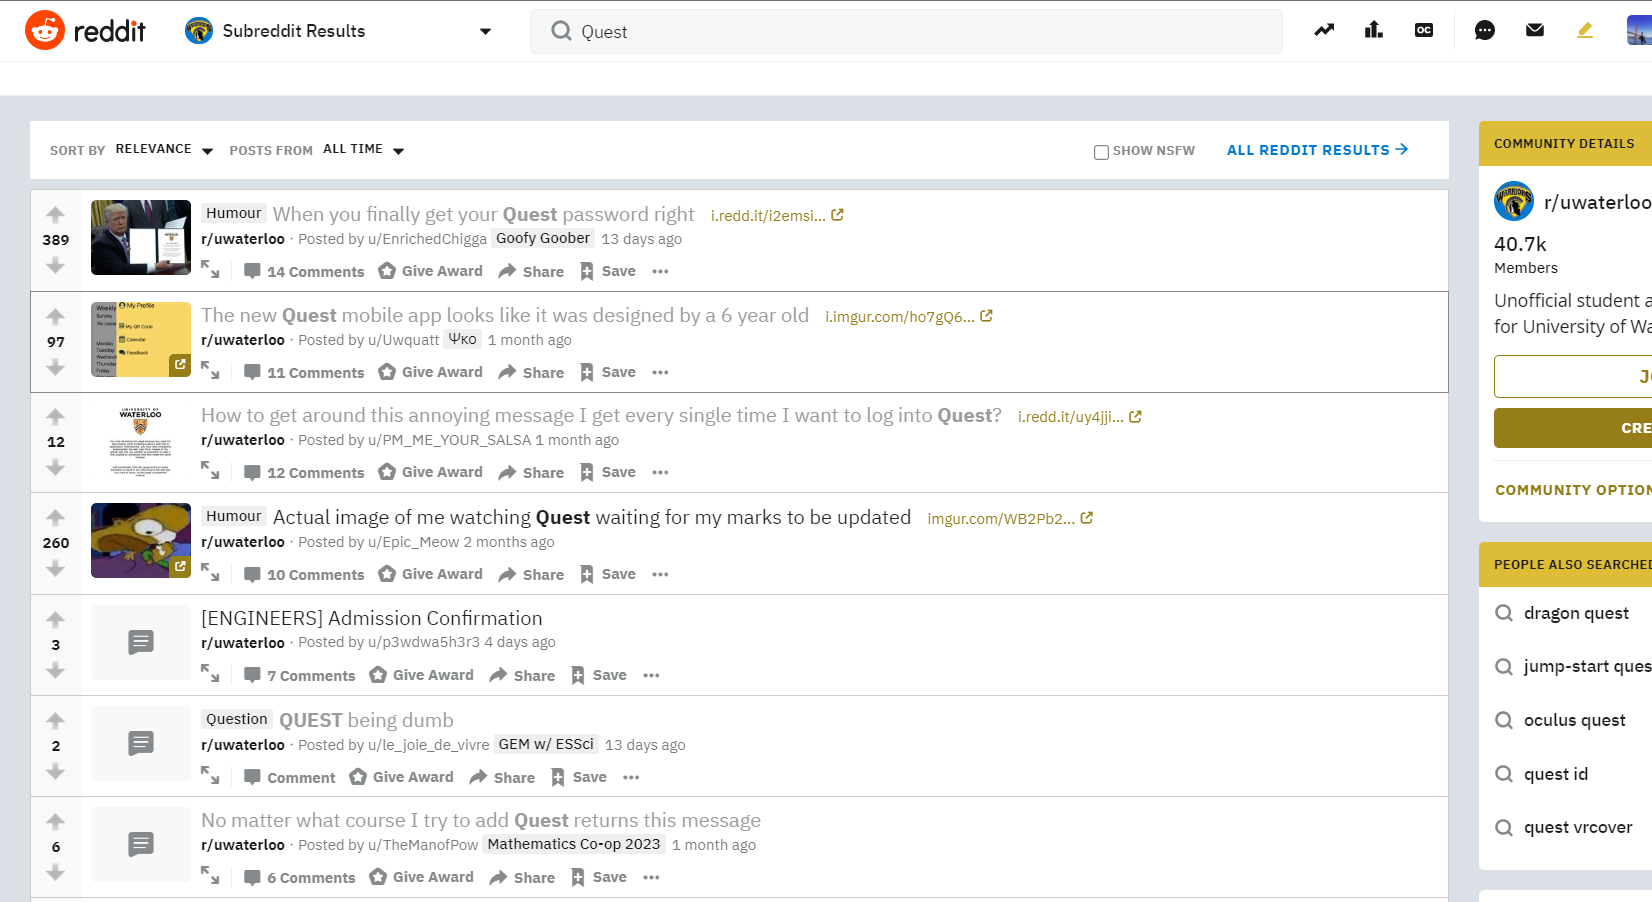
\includegraphics[width=1\columnwidth]{Reddit.png}
  \caption{Screenshot of Reddit search result with search term ``Quest'' under r/uwaterloo}
  \label{fig:figure1}
\end{figure}

\section{About Quest} \label{about quest}
\subsection{Introduction of Quest}
For readers who do not associate with UWaterloo, Quest is UWaterloo's Student Information System (SIS). The user groups of Quest can be identified and divided into three groups: applicants (future students), current students (undergraduate and graduate), and faculty and stuffs. Quest is available for access on both desktop computers and mobile devices. In this case study scenario, Yilun would be examining Quest as a UWaterloo's current (graduate) student who typically uses Quest on his desktop computer. This scenario is selected based on the author's graduate student status and a small survey on other UWaterloo students asking on which platform they use Quest the most commonly. According to the UWaterloo Quest official website, features for current students of Quest on the mobile devices and the desktop computer are separated \cite{b1}. Most features are listed the same on both platforms, with two exceptions: tuition account summaries, tuition tax receipts are listed only as of the mobile devices features. However, tested by Yilun in reality, all features available on mobile devices can also be accessed on desktop computers. So the features of Quest includes: enroll in courses, change personal contact information, and view class schedule, tuition fees, tuition account summaries, tuition tax receipts, financial aid, and student record information \cite{b1}. Those can be identified as the main UCa of Quest for current students. 

\subsection{New Update in February} \label{new update}
Quest got an update on February 2019. From now on, old Quest refers to Quest before the February update, and new Quest refers to Quest after the update. According to the news by UWaterloo's Registrar's Office, the new Quest provides users with a new navigation structure and a tile-based layout on its homepage, as shown in Figure~\ref{fig:figure2} \cite{b4}. The new Quest is intended to offer users: an improved workflow; enhanced navigation options; reduced clicking; a modern look and feel; easier access to help resources; and an experience that aligns with that of Quest Mobile \cite{b4}. Comparing to the old Quest's Student Center Homepage (SCH), as shown in Figure~\ref{fig:figure3}, the new Quest has a more condensed and simplified layout. Yilun has experienced both the old and the new Quest. So he found the update interesting and exciting, thinking it would be a whole new experience with Quest.

\begin{figure}[htdp]
%%\centering
  \centerline{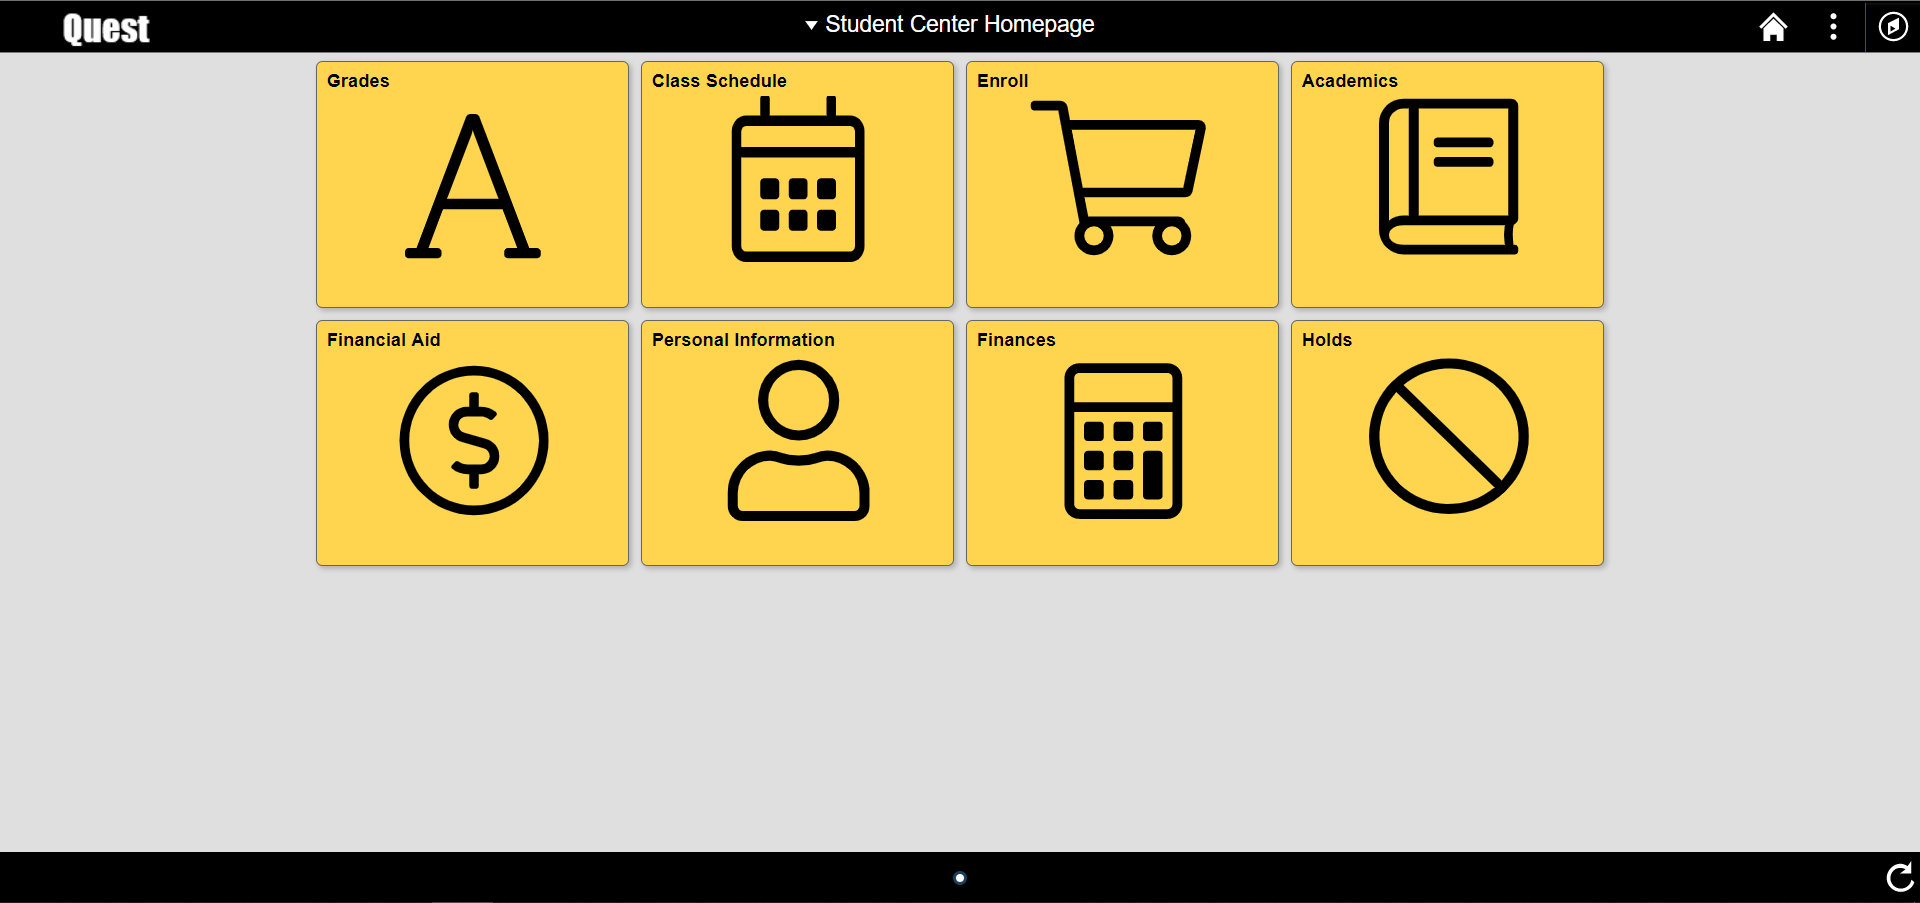
\includegraphics[width=1\columnwidth]{Student_Center_Homepage.png}}
  \caption{Student Center Homepage (SCH) of the new Quest}
  \label{fig:figure2}
\end{figure}
\begin{figure}[htdp]
\centering
  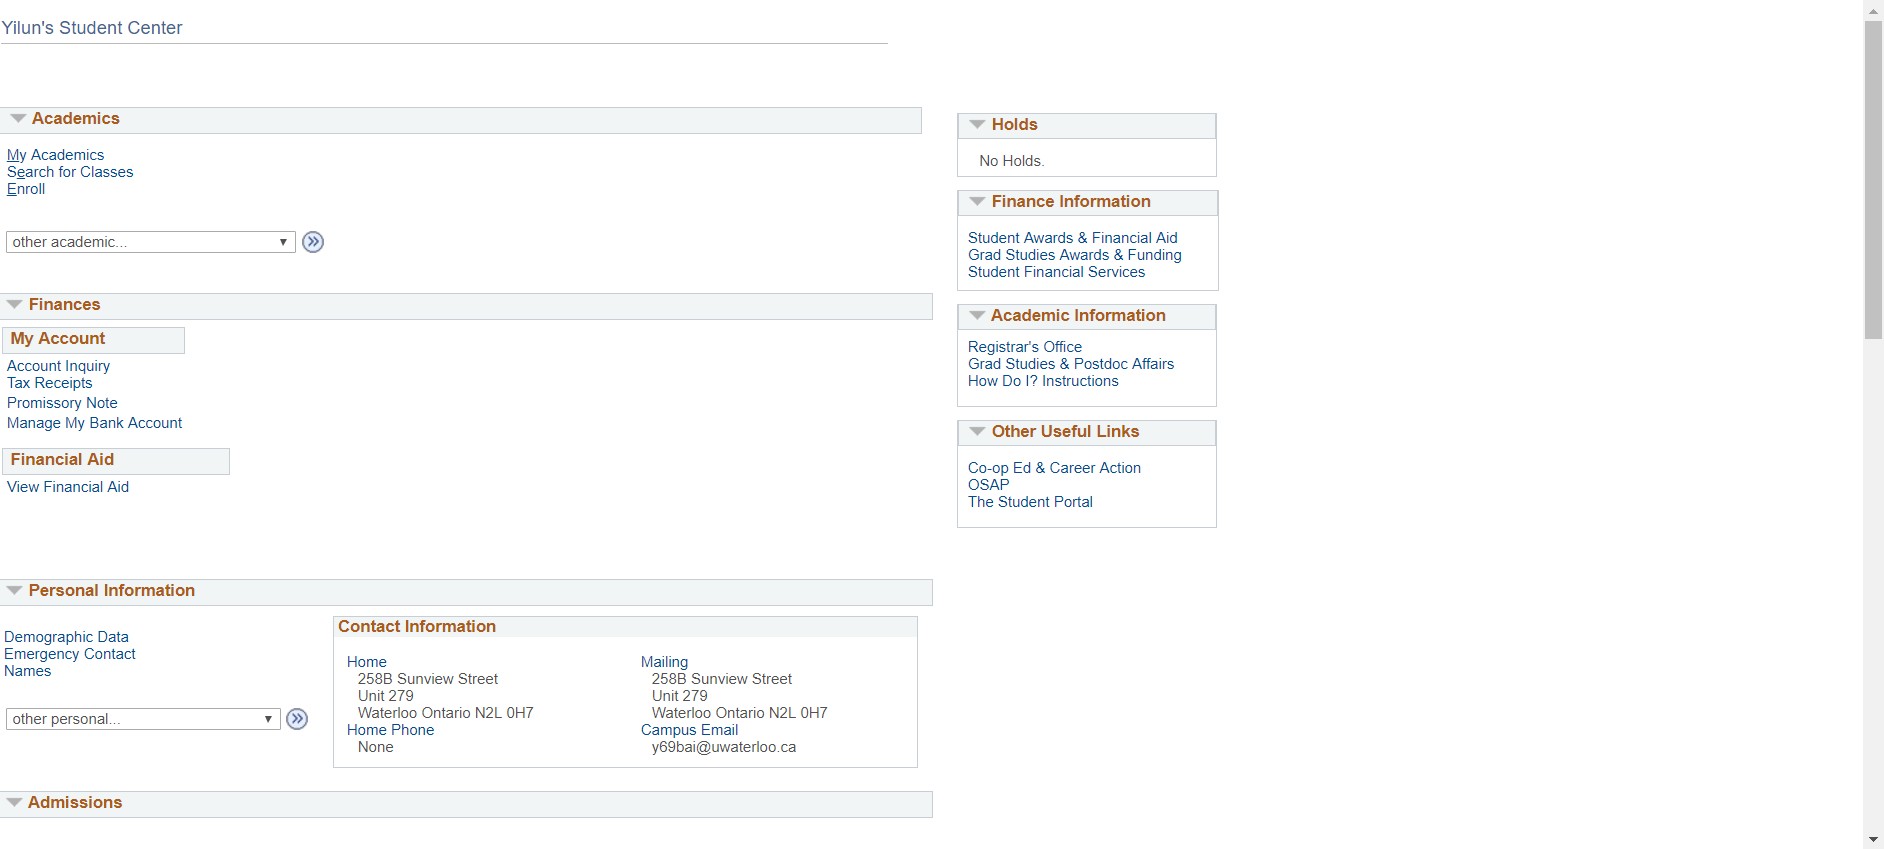
\includegraphics[width=1\columnwidth]{Old_student_center_homepage.png}
  \caption{Student Center Homepage (SCH) of the old Quest}
  \label{fig:figure3}
\end{figure}

However, when he got to use it more thoroughly, this update did not seem to be that much of an improvement. Yilun found that the actual site content and how users use those pages remained exactly the same. As shown in Figure~\ref{fig:figure4}, both versions of Quest are on the same class enrollment page. The new Quest on the right has the same internal page as the old Quest on the left. The only difference is the new Quest has a Left Panel that copies the same navigation tab originally located horizontally on the top, and a top banner that allows users to go back to the SCH and shows the name of the current page.

\begin{figure}[htdp]
\centering
  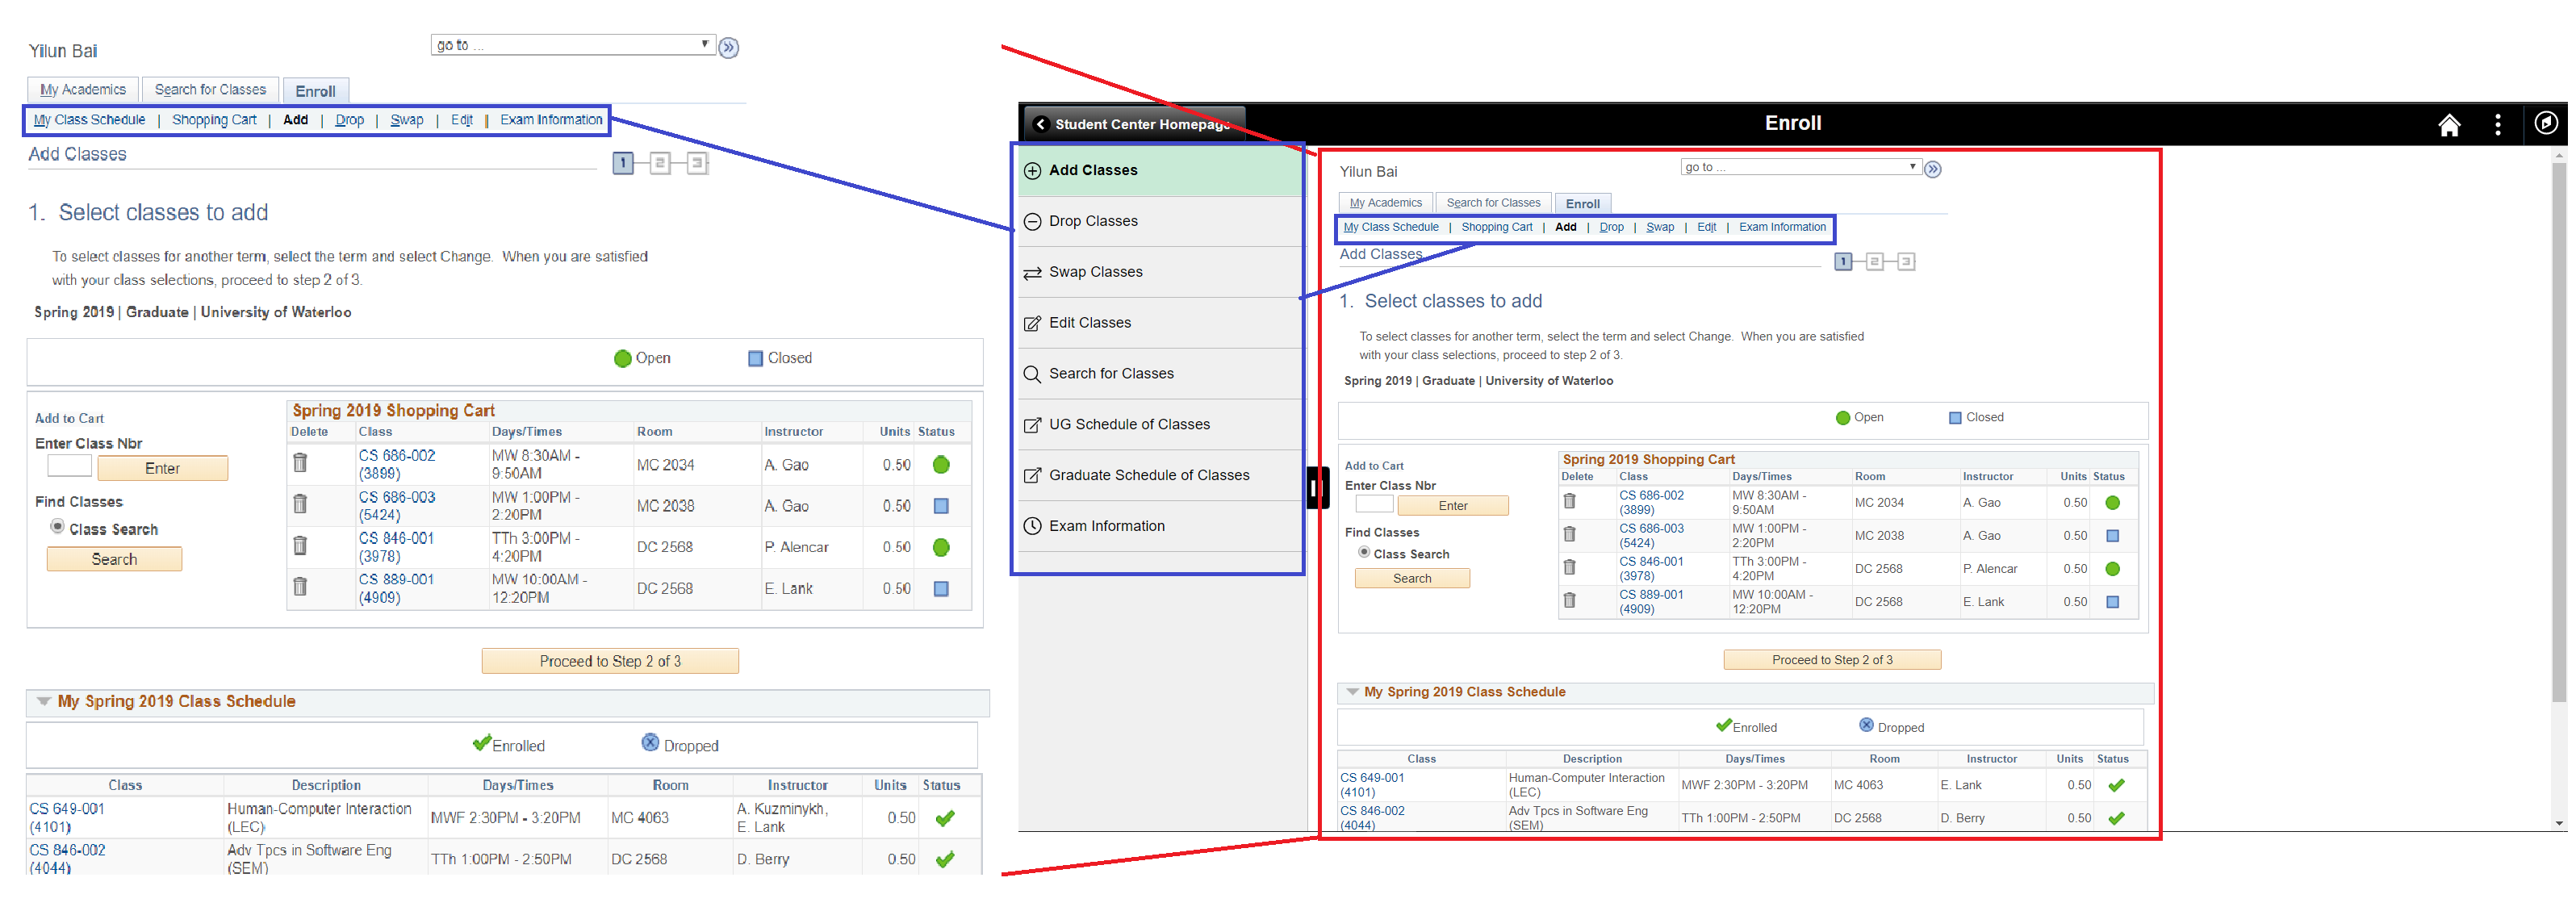
\includegraphics[width=1\columnwidth]{a.png}
  \caption{The actual site of Quest remains exactly the same}
  \label{fig:figure4}
\end{figure}

\section{Case Study on Quest}  \label{case study on quest}
\subsection{Conversation with Quest People}
In order to get an insight on Quest and learn more about the development side of things, Yilun decided to communicate directly with the Quest people. Through research, he found out that Quest is developed and maintained by the UWaterloo's Student Information System Program, which has this steering committee that meets regularly to review priorities relating to Quest \cite{b5}. Therefore, Yilun sent out an email to three of the committee members, asking if there was any Software Requirement Specification (SRS) document to look at or any other requirement engineering related insight on the development of Quest. 

One of the committee members, Daryl, who is the director of Enterprise Resource Planning and Data System, responded. He pointed out that the Quest system is built based on Oracle PeopleSoft Campus Solution System which is a packaged application used by many other schools as well \cite{b6}. It was originally implemented at UWaterloo in 2001 and has evolved based on the adding features by Oracle and the requirements from the university \cite{b5}. The update in February is the adoption of the Fluid interface from Oracle. At the university, they did not document detailed requirements because the interface is a standard offering and there are limited abilities to customize the interface. The Quest team thinks it is highly beneficial to stay with delivered functionality for packaged applications. So the update choices in this February were largely about the order of tiles, icons and applying branding. The primary effort for that initiative was consulting with each user group (students, staff, faculty) to understand the optimal tile layout for their home screen. These consultations reviewed prototypes and changes were implemented based upon feedback. Given the agile nature, Yilun did not get any documentation shared by the Quest team.


\subsection{PeopleSoft Fluid versus Quest}
Since there was no documentation from the university side, Yilun had to go visit this Oracle Fluid website to find sources to understand how Quest was designed for this update. On the Oracle website, Yilun managed to find the PeopleSoft Fluid UX Standards, which is a document for designers and developers containing information about key functionality to create a usable, consistent, efficient and productive experience for users \cite{b7}. 

Reading through the standards document, Yilun found examples that are very similar to the new Quest. For example, the Quest SCH tile showed previously in Figure~\ref{fig:figure2} looks really similar to the Fluid Homepage example, as shown in Figure~\ref{fig:figure5}. Both have this tile-based layout. However, noted that in the Fluid Homepage example, some of the tiles are live tiles, which contains live data, compared to the static tiles on the Quest SCH. The use of live tiles allows users to view at-a-glance live informational data for decision making and monitoring, in addition to being able to drill-down to the transaction and perform certain tasks. A good use of live tiles on the Quest SCH can be very useful. For example, the Finance tile can have live data on the tuition charge balance and the Grades tile can have live status on the availability of grades. 

\begin{figure}[htdp]
\centering
  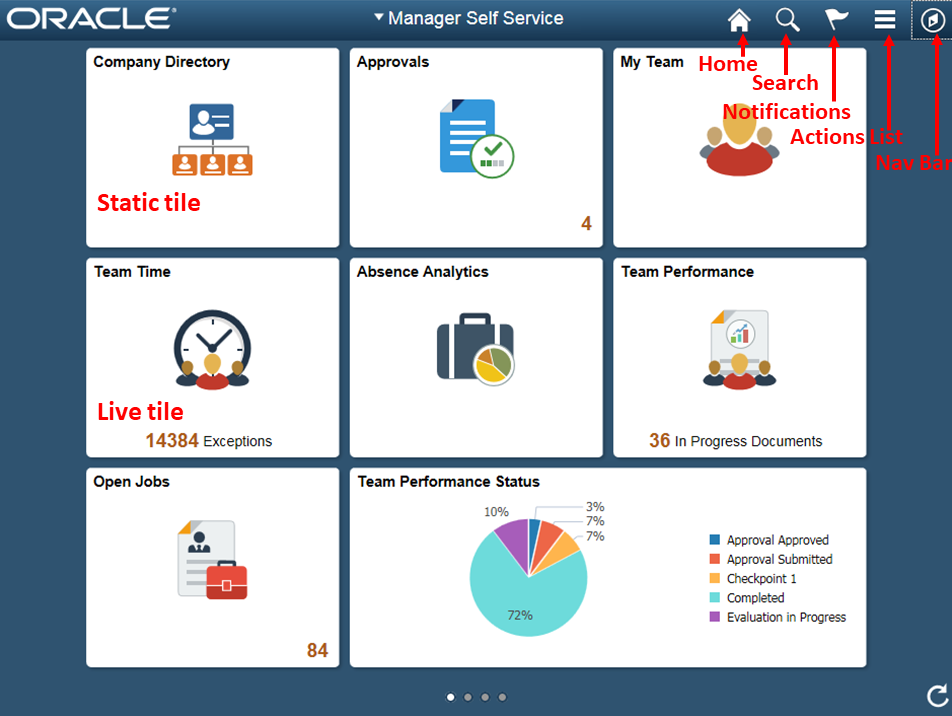
\includegraphics[width=1\columnwidth]{Fluid_homepage_example.png}
  \caption{Fluid UX example Homepage \cite{b7}}
  \label{fig:figure5}
\end{figure}

Also on the top right corner of the Homepage for both Fluid and Quest, there are icons in the top banner, as shown in Figure~\ref{fig:figure5}. In the Fluid example, there are Home, Search, Notifications, Actions List, and Nav Bar. On Quest, there is only Home, Actions List and Nav Bar. The search feature and the notification system are abandoned by the Quest team. As for the Nav Bar implemented by Quest, there is only a Recent Places folder and a Sign Out button. Unfortunately, the Recent Places feature on Quest does not work, showing blank no matter which page you tap on. The Actions List icon is also basically useless with only a redundant Sign Out option.

On to the actual site, the user interface layout is also very similar between the Fluid example and Quest. As shown in Figure~\ref{fig:figure6}, both pages are on the personal detail/information page. A Left Panel is presented for quick navigation. However, since new Quest kept the exact same internal page, the left panel now contains the same navigation feature as the traditional, horizontal display of tabs on the internal page. The new Quest offers users the ability to show and hide the left panel for larger screen space by tapping the black tab on the side of the left panel. But doing that diminished the point for this navigation-focused update of Quest even more. 

\begin{figure}[htdp]
\centering
  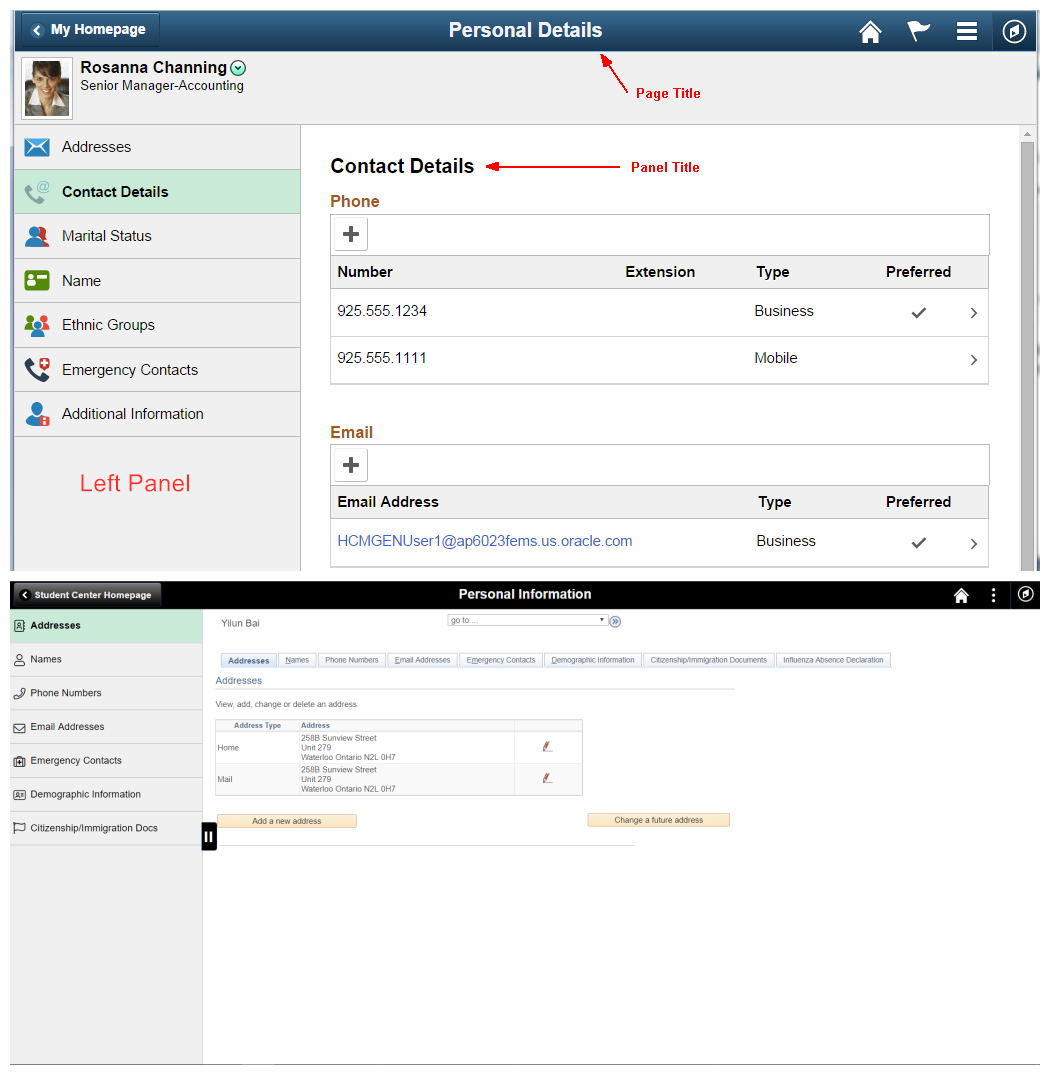
\includegraphics[width=1\columnwidth]{Personal_detail.png}
  \caption{Fluid UX example Personal Detail page (top) versus new Quest Personal Information page (bottom) \cite{b7}}
  \label{fig:figure6}
\end{figure}


Overall the updated new Quest is more like a hybrid child birthed by Fluid UI and the old Quest, or in other words, a semi-finished product. Only the SCH and the navigation around the pages are changed. There are no extra features or feature functional improvements since all the internal pages remain the same.

\subsection{Follow-ups With the Quest People}
With those questions in mind, Yilun then sent a follow-up email back to Daryl, asking the reason behind not to implement Quest fully based on the PeopleSoft Fluid UX Standards. Daryl replied once again with insight.

When the team at UWaterloo implemented Quest based on purchased PeopleSoft Campus Solution, it was still evolving and Quest was heavily customized.  Over time, Oracle has enhanced the product but it is a lot of work for the Quest team to remove the customization and replace them with delivered functionalities. The Quest team don't prioritize those de-customization initiatives highly unless they add new features to benefit the campus community and provide benefit.  Whenever they take on a project in an area they try to de-customize it as they go as they have done recently with the SCH and are working on for Admissions.
 
Customized pages don't work well with Fluid so they cannot move all pages to that design standard without a lot of work for little benefit. They moved the navigation and home page to fluid because it improved the user experience and lets us use many of the newer features without having to de-customize the whole thing. Oracle promotes Fluid+ because it helps fill this common challenge across clients.


\subsection{Analysis of the old and new Quest}
In order to see if the February update of Quest actually achieved its goals described in Section \ref{new update}, Yilun decided to perform a series of UCa and USc task-based testing on both the old and the new Quest.

\subsubsection{Click Testing}
The major focus on this update is on enhancing navigation options and reduce clicking. Therefore, Yilun performs a variation of click testing to see if the new Quest navigates better than the old Quest. Click testing is a traditional method of evaluating the prototype design by examines what user clicks on first in order to complete a given task [8]. Users are almost twice as likely to succeed in a task if the first click was down the right path [8][9]. Yilun's click testing is conducted on a task-by-task basis. Tasks are selected based on the frequently used UCa listed on the official Quest website. In this click testing, Yilun also examined the number of clicks for users to navigate to a particular page to see if the new Quest indeed reduced the number of clicks. Since the new Quest also has the old Quest's horizontal navigation tab on the internal pages alongside with the left panel, in this click testing for the new Quest, Yilun shall only use the newly added navigation tabs instead of the initial ones. 

Here is an example of the procedure of this click testing, as shown in Figure~\ref{fig:figure7}. The first task is the use case for checking grades. Users like Yilun would perform this use case on a regular basis at the end of every term. On the old Quest page, starting from the SCH, Yilun would click on ``My Academics'' under the Academics category. Then the old Quest would direct Yilun to the ``View My Grades'' tab under the ``My Academics'' tab, where Yilun is presented a list of terms to select from. The number of clicks up until this point is 1. On the new Quest page, also starting from the new SCH, Yilun can see a tile named ``Grades''. And by clicking on the ``Grades'' tile, Yilun will be directed to the same ``View My Grades'' tab under the ``My Academics'' tab, with an additional left panel and a top bar. Then, in order to view the grades of a particular term, Yilun would perform the same action as he would on the old Quest page. Therefore, the number of clicks for this task on the new Quest is also 1. It is a draw between the old and the new Quest on this task.

\begin{figure}[htdp]
\centering
  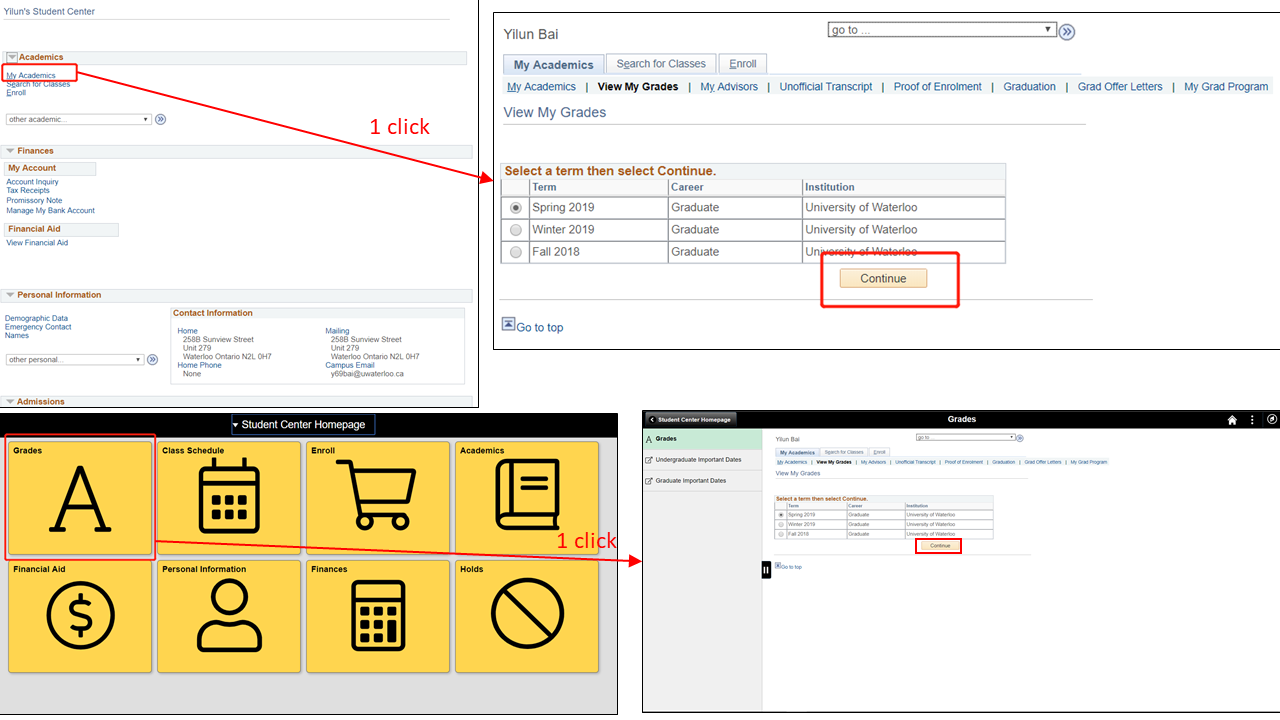
\includegraphics[width=1\columnwidth]{click_grades.png}
  \caption{Click Testing on the old Quest (top) and the new Quest (bottom)}
  \label{fig:figure7}
\end{figure}

The same procedure of click testing is performed on other tasks (UCa), including view class schedule, change phone number, check unofficial transcript, check tuition, class enrollment - add courses. Table ~\ref{tab1} lists the number of clicks to perform a certain task on both old and new Quest.The new Quest has a slight edge over the old Quest in terms of a less number of clicks.

\begin{table}[htbp]
\caption{Number of clicks to perform a task starting from SCH}
\begin{center}
\begin{tabular}{|c|c|c|c|}
\hline
\textbf{}&\multicolumn{2}{|c|}{\textbf{Number of Clicks}}&\textbf{} \\
\cline{2-3} 
\textbf{Task (UCa)} & \textbf{\textit{Old}}& \textbf{\textit{New}} & \textbf{Winner} \\
\hline
Check grades & 1 & 1 & Draw \\ \hline
View class schedule & ? & 1 & New \\ \hline
Change phone number & 1 & 2 & Old \\ \hline
Check unofficial transcript & 3 & 2 & New \\ \hline
Check tuition & 1 & 1 & Draw \\ \hline
Class enrollment & 2 & 1 & New  \\ \hline
\end{tabular}
\label{tab1}
\end{center}
\end{table}

Two outliers occurred in the click testing. When performing view class schedule, Yilun failed the first click testing on the old Quest and eventually got lost in the system. The class schedule seems to be an academic thing, but there is no class schedule tab on the SCH. Yilun then clicked on the ``My Academics'' tab to explore more options. But there was still no class schedule sub-tab under it. Yilun found a ``My Academics'' sub-tab under the ``My Academics'' tab and click on it, only to bring him to the ``My Academics'' home page. Eventually, Yilun had to go back and explore under other categories. On the new Quest, however, there is a ``Class Schedule'' tile right on the SCH. Yilun only needed 1 click to perform this task. Turns out, the class schedule is not under the ``My Academics'' tab but under the ``Enroll'' tab. This showed that the navigation tab hierarchy is not well organized. 

Another outlier occurred when performing the change phone number task. On the old Quest SCH, there is a ``Home Phone'' tab under the ``Personal Information'' category with detailed information on display. Yilun can click on the ``Home Phone'' tab to go directly to the ``Phone Numbers'' page to complete the task. Whereas on the new Quest, the ``Personal Information'' tile would bring Yilun to the ``Addresses'' page under the ``Personal Information'' tab, where Yilun needed another click on the left panel to go to the ``Phone Numbers'' tab. The old Quest wins this task over the new Quest because it displayed more information than the new Quest. In order to achieve a simplicity feel of the tile-based homepage design, the new Quest had to eliminate certain informative contents originally on the SCH.

All the testings above are starting from the SCH. But what if the user scenario is when a user is on a sub-page and wants to navigate to another sub-page under a different category? Then, the USc is set to navigate from class schedule to tuition page; from tuition to emergency contact page; from demographic data to class enrollment page; from class enrollment to tax receipt page. Table ~\ref{tab2} shows the number of clicks to perform those tasks (USc) on both versions of Quest. Through testing, Yilun found that on both versions of Quest, users have to first navigate back to the SCH and then navigate from there. There is no direct navigation option for users to go to a specific page in another category. The old Quest performed poorly in those USc since the only way to go back to the SCH is through its drop-down selection list navigation method. As for the new Quest, the back button on the top left corner always brings users back to the SCH by only 1 click.

\begin{table}[htbp]
\caption{Number of clicks to visit a sub-page under a different category}
\begin{center}
\begin{tabular}{|c|c|c|c|}
\hline
\textbf{}&\multicolumn{2}{|c|}{\textbf{Number of Clicks}}&\textbf{} \\
\cline{2-3} 
\textbf{Task (USc)} & \textbf{\textit{Old}}& \textbf{\textit{New}} & \textbf{Winner} \\
\hline
Class schedule to Tuition & 4 & 2 & New \\ \hline
Tuition to Emergency contact & 4 & 3 & New \\ \hline
Demographic data to Class enrollment & 5 & 2 & New \\ \hline
Class enrollment to Tax receipt  & 4 & 3 & New \\ \hline

\end{tabular}
\label{tab2}
\end{center}
\end{table}

\subsubsection{User Interface Design}
One of the other goals for the February update of Quest is to provide a more modernized and user-friendly experience. So let's look at Quest from a user interface perspective. 

The Rule of Thirds is a very well known term in user interface designing for websites. The idea is to place a simple grid overlay which is divided equally into thirds both horizontally and vertically onto the web page, as shown in Figure~\ref{fig:figure8} \cite{b10}\cite{b11}. The points where the lines cross are the focus points. Key elements should be placed near those focus points or along the lines since those areas are to where the eye will automatically fall towards.  

\begin{figure}[htdp]
\centering
  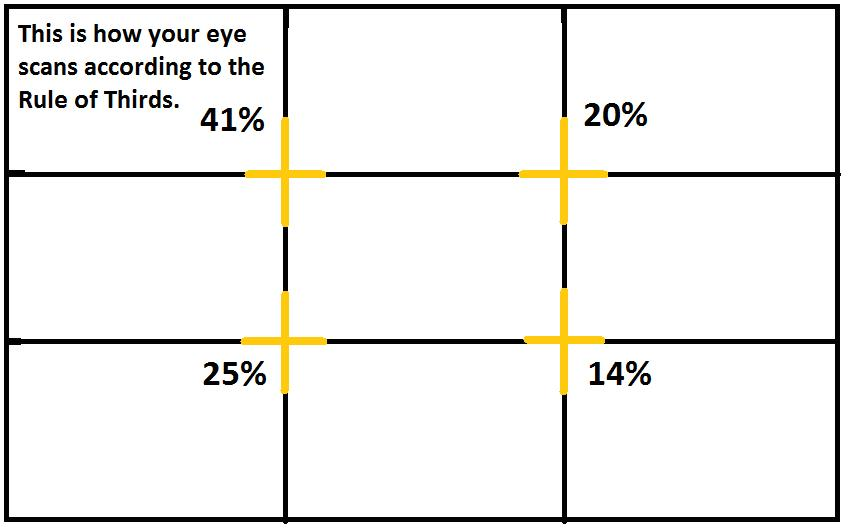
\includegraphics[width=1\columnwidth]{rule_of_thirds.jpg}
  \caption{Rule of Thirds \cite{b10}}
  \label{fig:figure8}
\end{figure}


If we apply this Rule of Thirds on the SCH of both the old and the new Quest, as shown in Figure~\ref{fig:figure9} and Figure~\ref{fig:figure10}, we can see that none of the important information on the old Quest is even near the four focus points. Readable contents are all densely assembled on the left side of the screen, resulting in this awkward-looking and unhandy SCH. The new Quest, however, has a very symmetrical and centralized tile-based layout. All the information is either around the focus points or along the lines. If we apply this Rule of Thirds onto the internal pages, as shown in Figure~\ref{fig:figure11}, the left panel of the new Quest actually helps to push the important information more towards the middle of the screen and those focus points compared to the old Quest. 

\begin{figure}[htdp]
\centering
  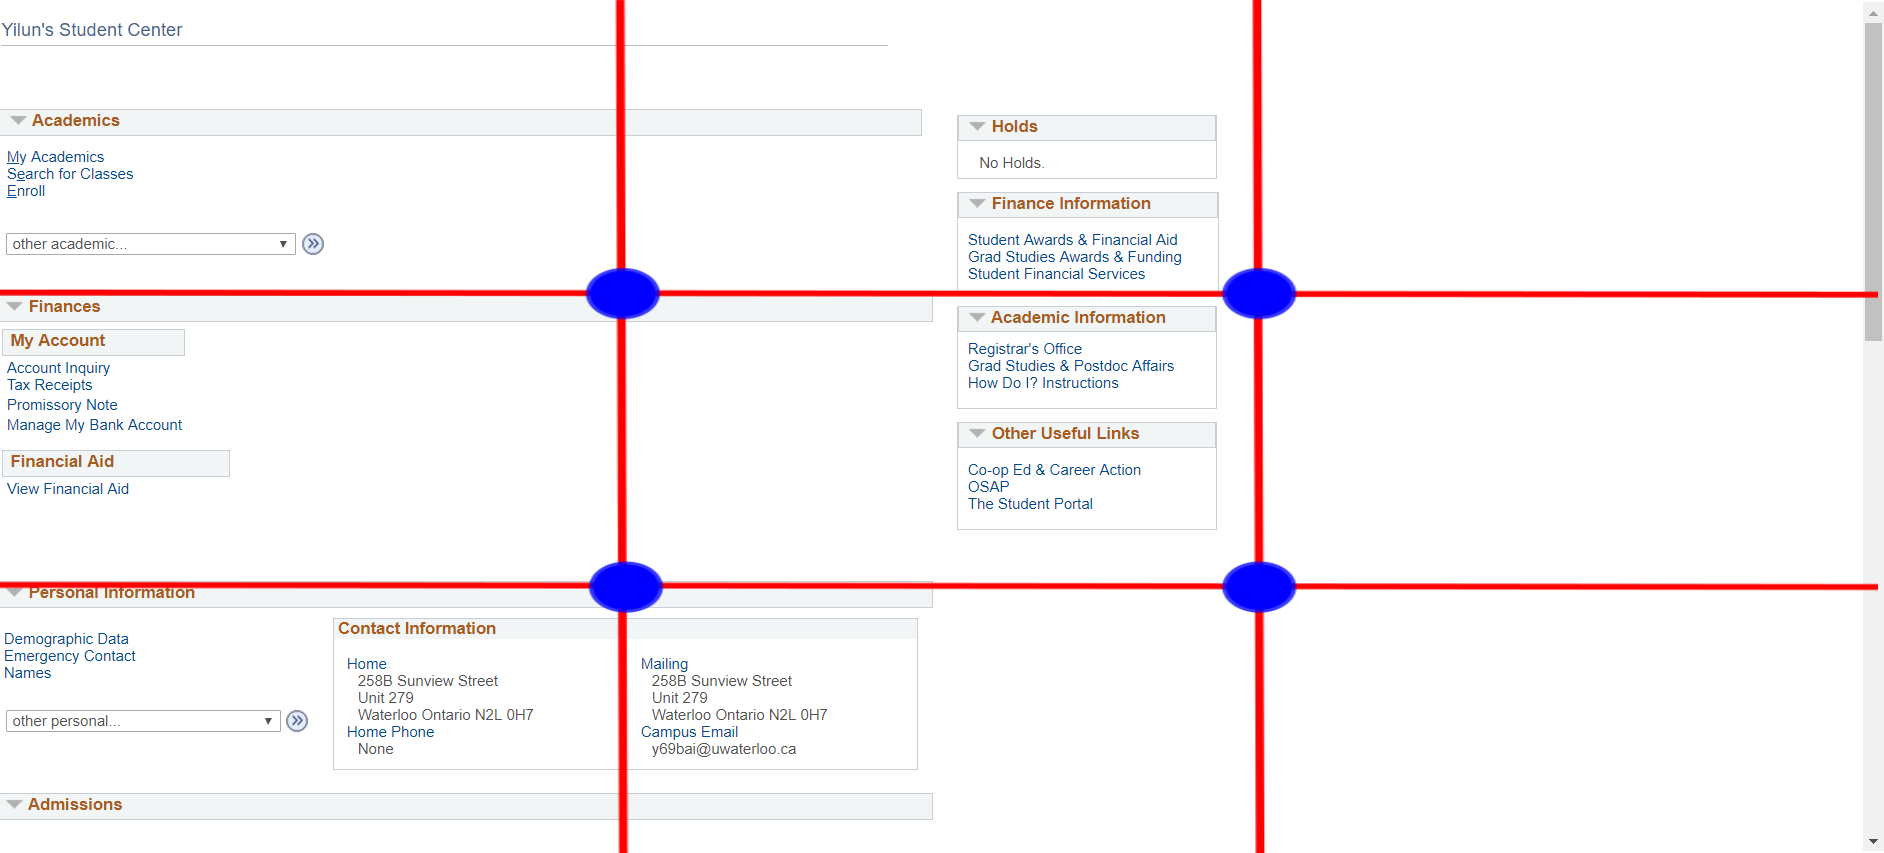
\includegraphics[width=1\columnwidth]{Old_student_center_homepage_full_grid.png}
  \caption{Applying Rule of Thirds on the old Quest SCH}
  \label{fig:figure9}
\end{figure}
\begin{figure}[htdp]
\centering
  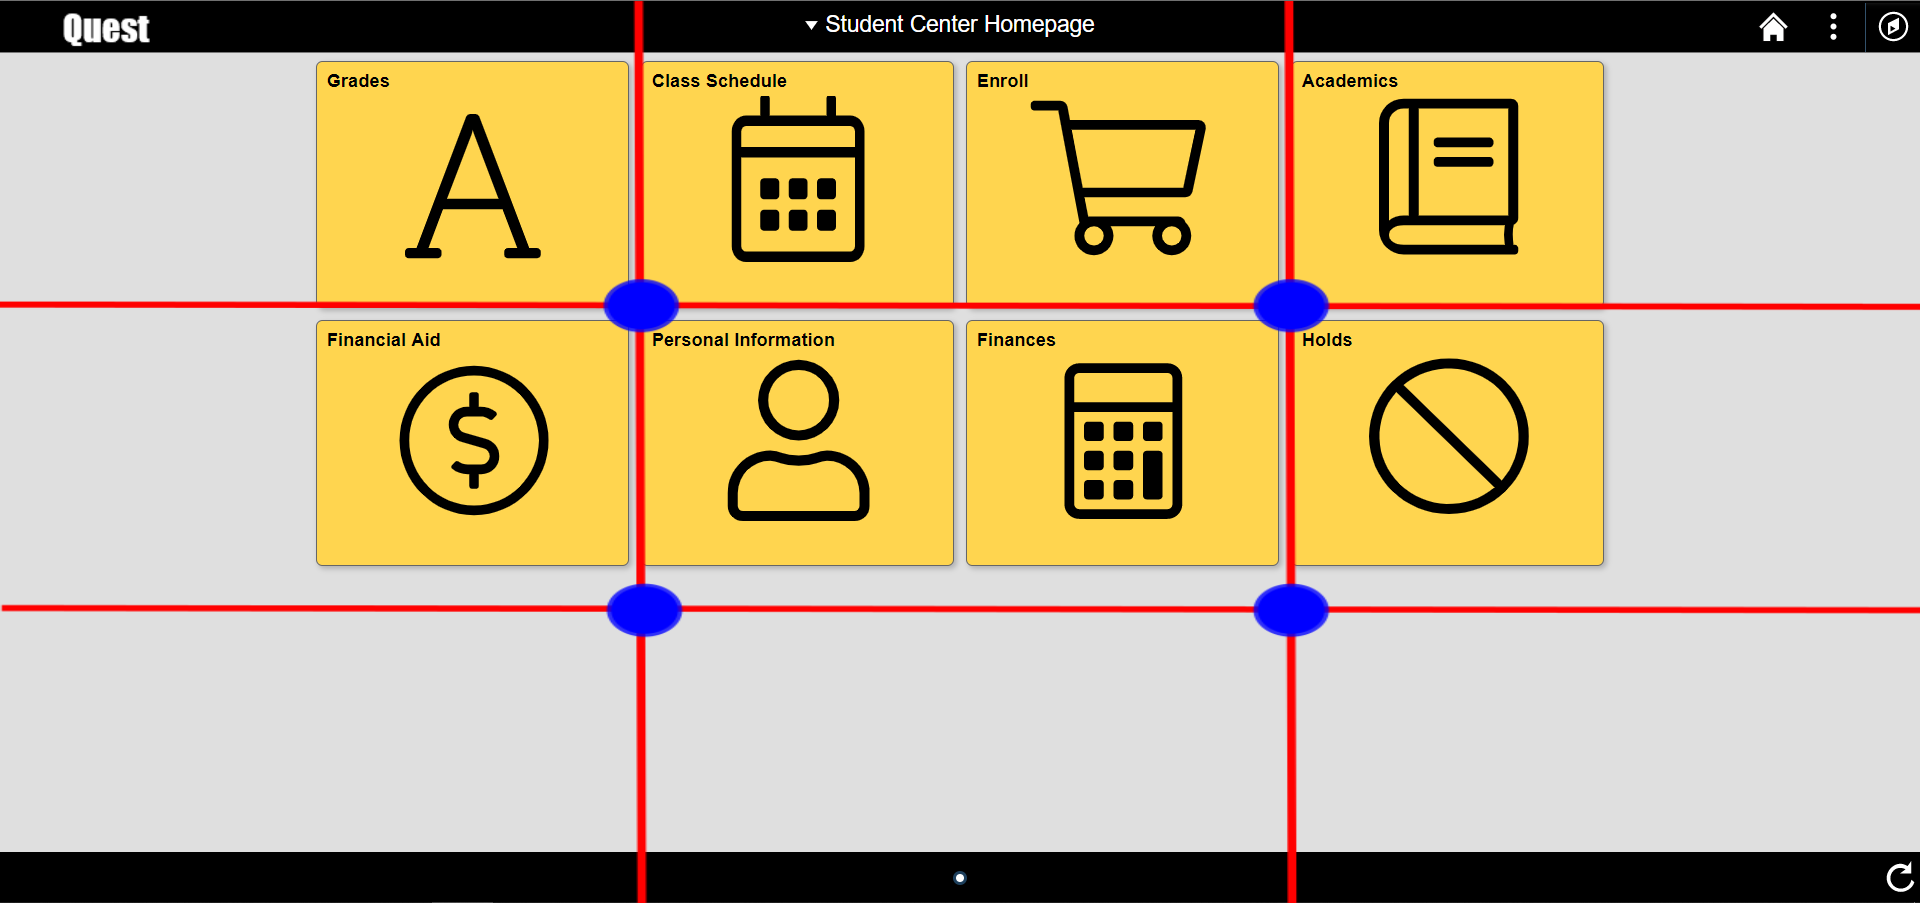
\includegraphics[width=1\columnwidth]{Grid_Student_Center_Homepage.png}
  \caption{Applying Rule of Thirds on the new Quest SCH}
  \label{fig:figure10}
\end{figure}
\begin{figure}[htdp]
\centering
  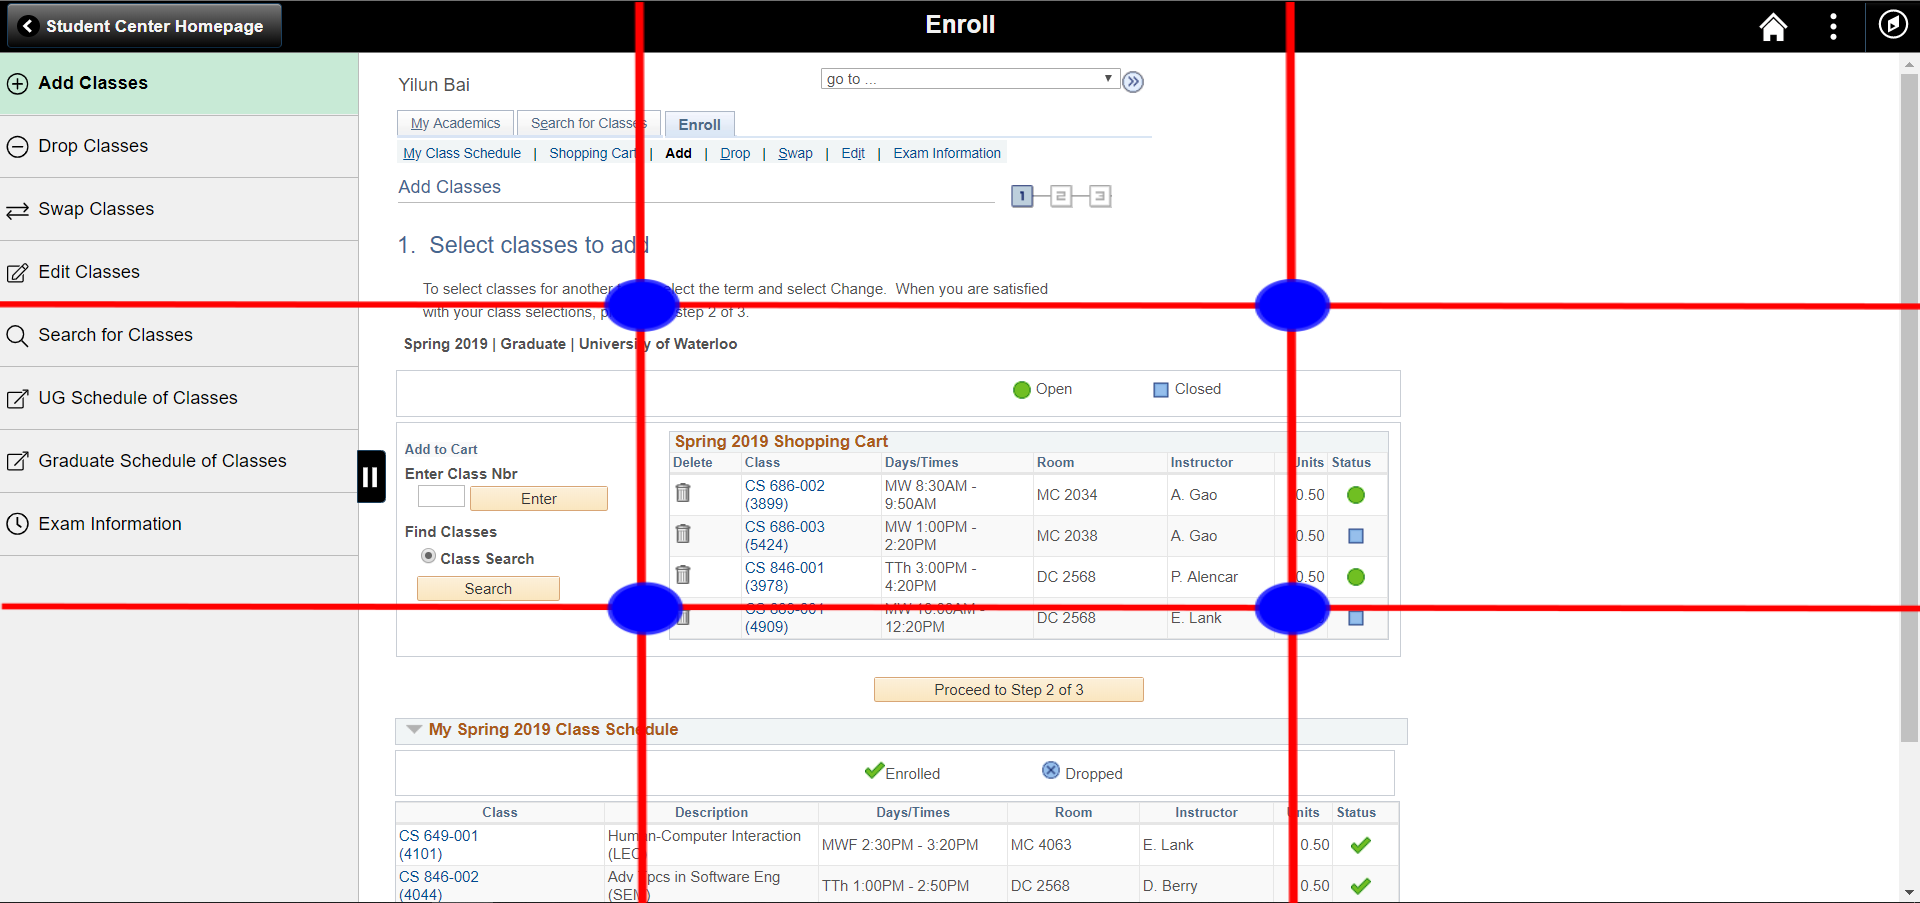
\includegraphics[width=1\columnwidth]{grid_enroll_page.png}
  \caption{Applying Rule of Thirds on the new Quest class enrollment page}
  \label{fig:figure11}
\end{figure}


The use of free space is also a very important technique in UI design. Smartly used free spaces can make important elements stands out, organize content in the layout through proximity, improve user comprehension, and direct the user through the blocks of content shown. There are two kinds of free space, micro and macro \cite{b12}. Small gaps between design elements are micro free space. Large space between major layout elements and the space surrounding the design layout are macro free space. If we look back to the old Quest SCH in Figure~\ref{fig:figure9}, we can see there are two giant free space, one in the middle, the other on the right. They are macro free spaces that are misused and misplaced, taking up over half of the page size. As for the internal page on the new Quest in Figure~\ref{fig:figure11}, the free space on the right peripheral is smaller compared to the old Quest without the left panel shifting the content to the right, but still massive. 

\subsubsection{Functionality}
Since there is no change in the internal page of Quest for this February update, existing functionality problem still exists. One of the most discussed and complained UCa is the class enrollment process which all students like Yilun would use multiple times and rather frequently every term until the end date to change class schedule. In the current class enroll process, users need to perform 3 steps: 1. Select classes to add - put in the shopping cart; 2. Confirm classes; 3. Finish enrolling. However, during the process, only a list view of the detailed pending courses and enrolled courses is shown. Often times users encounter failures due to time conflicts with other selected or existing courses. And users need to go back to change the shopping cart and try again. Users need to manually check on the time detail and cross-reference manually to ensure there is no time conflict. This is especially true for undergraduate students who takes a lot of courses which have different section offerings. The usability of this functionality is not well designed without a visualization on the schedule for selected potential courses.


\section{Problems Identified and Suggested Solutions in Summary}  \label{probelms and sulutions}
All problems identified up until this point is summarized into the following list:
\begin{itemize}
\item The page/section/tab hierarchy is not well organized, e.g. Class Schedule can be viewed under Enroll tab, not My Academic tab; My Academic sub-tab under My Academic tab.
\item The left panel navigation combine with the original top bar page navigation is redundant; Some also not consistent.
\item The left panel and the page name in the top banner do not follow the changes of the pages if user use the old ``Go to'' navigation instead of the left panel.
\item Non-function icons in the top banner - Action List and Nav Bar do basically nothing, e.g. Recent Places in the Nav Bar does not actually record on which page users have been.
\item Both versions of Quest couldn't handle efficient transfer from sub-page to another sub-page without going back to the SCH, e.g on the tuition page, users want to go straight to class enrollment page.
\item Large free spaces on the right side of the page are wasted on basically every page.
\item Limited information displayed on the SCH.
\item Some feature workflow is lengthy, i.e. the class enrollment 3 step process. Adding a class in the shopping cart does not reflect in the calendar view.
\item Overall UI lack of consistency – black and gold only appears on the SCH but nowhere else.
\end{itemize}

\newline
And suggestions are provided to either solve existing problems or make Quest better.
\begin{itemize}
\item SCH tiles customization - User should have the ability to add, remove, or rearrange tiles on the SCH for quick access.
\item A schedule builder in calendar view should be provided - whenever users selected a potential course to add to their class schedule, the calendar view should reflect the relative changes on the existing schedule in real time.
\item Search functionality - PeopleSoft Fluid has a search bar in the top banner. Quest should keep it for in Quest searches or searching sites under uwaterloo.ca.
\item A new Quick Links widget can be added on the right side of every page - Users can add frequently visited page link. It allows user to jump between pages under different categories without going back to the Homepage and also makes use of the large free space on the right side of the page.
\item Automatic exam information update - final exam schedule, date, location, seat, etc. Quest knows the users class schedule and should extract and display exam information from the exam schedule PDF with no problem.
\item A notification system - PeopleSoft Fluid has a notification icon in the top banner. Quest should keep this functionality for notifying critical information, school updates (snow day, power outage), important due date (tuition, class enrollment/drop), exam date approaching, etc.
\item Make use of the live tiles on the SCH to display more information related within certain tiles could improve productivity.
A rework on the UI style of design to make the whole Quest more coherent.
\end{itemize}


\section{Discussion, Related Literature Review, and Lessons Learned}  \label{discussion and reviews}
As Daryl said, the adopting of new versions of software and new requirements from the university are the main challenges they're facing when providing maintenance for Quest. The use of immature software is one of the reasons that lead to a software project failure \cite{b13}. In this case, the immature software Quest used for development is the evolving Oracle PeopleSoft Campus Solution. Quest and Oracle evolve on their own paths and overtime the gap gets larger and larger. Quest is already a developed product that could not afford to shut down for maintenance for a long period of time since it is underused by tens of thousands of stakeholders on a daily basis. However, find and fix an error, adding new requirements, or adopting to new requirements in the post-delivery maintenance phase has a much higher cost than doing so in the early phases such as during the RE phase or analysis phase. As shown in Figure~\ref{fig:figure12}, the approximate relative cost to detect and correct a fault during the maintenance phase can be over 200 times more compared to during the requirements phase \cite{b14}. Therefore, it takes time for Quest to fully adopt to a new system standards (Fluid) and fixing existing and new problems along the way. But due to its monopoly nature, i.e. users have no other alternatives, Quest has to provide a mid-staged working product, as in the new Quest after the February update, to supply users' continuous usage until it reaches an optimal stage. Yilun would argue that when the cost of fixing problems get too large, it might be more efficient to abandon the current version and build everything from ground up, like what the University of Washington did with their SIS ``MyUW'' from 2016 to 2018 \cite{b15}\cite{b16}.

\begin{figure}[htdp]
\centering
  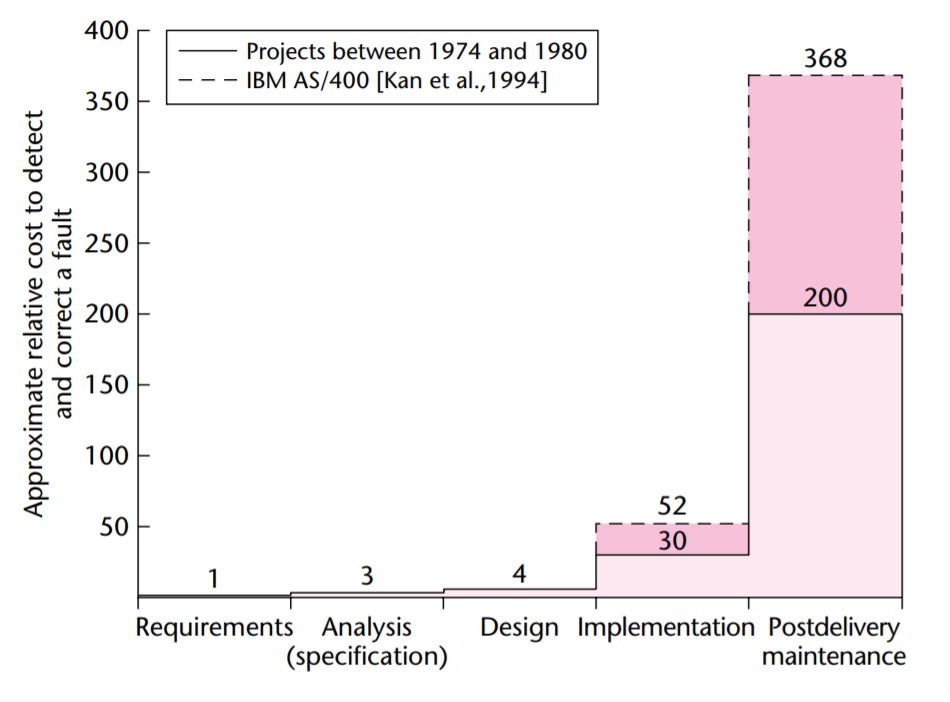
\includegraphics[width=1\columnwidth]{cost.png}
  \caption{Cost to fix fault under different development phases \cite{b14}}
  \label{fig:figure12}
\end{figure}

In the commercial circumstance, UX design plays a huge role which cannot be ignored. Since competitors would take the market share if your design of a product cannot make the users satisfied \cite{b17}. However, in this case of the Quest, users, i.e. the students and faculties, don't really have an alternative. All user groups have no choice but to learn and adapt to Quest despite its problems, instead of switching to an alternative because there isn't any. This causes poor user experiences and productivity. Minor bugs are left without resolving by the development and maintenance team, mainly due to the fact of lacking motivation and initiative from the competitive market. Therefore, it is crucial for users to make their voice heard by the developers. Under this circumstance, the only way Quest can improve to meet users' needs is through developers constantly gathering user requirements from all stakeholders throughout the product development and maintenance cycle \cite{b17}. 

Agile RE has the benefit of having lesser documentation, quick feedback and prototyping which is suitable for this Quest development scenario \cite{b18}. According to Daryl, they are using the agile development strategy by trying to de-customize the old Quest area by area to adopt the delivered functionalities from Fluid as they go. Hybrid development models with a combination of user-centered design need to be applied aiming to deliver suitable UX. In a paper of which the authors conducted a systematic literature review on agile RE address to stakeholder and user involvement, they identified four methodologies, including Human-Centered Design, Design Thinking, Contextual Inquiry, and Participatory Design, that were integrated in agile software development with the aim to increase the knowledge about user needs \cite{b19}. They also identified a broad range of different methods that can be used in agile software development. Key artifacts are also identified for the documentation of requirements that are used in Agile RE: User stories, prototypes, UCa, USc and story cards \cite{b19}. This can be a good lesson for the Quest team on future development and evaluation which should involve more users from different user groups in the process. 

During the case study, Yilun found the field of RE and HCI shares some common grounds. They are both design disciplines that guides software system development. They also have shared processes and representations, promoted in different ways, such as scenario-based design, user-centred design, agile methods and iterative design cycles with testing and evaluation \cite{b20}. Just like reliability, safety, and security  must be specified from the beginning, a good user interface also cannot be programmed in later. It needs to be required from the beginning of the design process \cite{b21}. An executable user interface should be rapidly developed for requirements clarification on both the user interface and on the functionality of the application \cite{b21}. Prototyping is one of the most adopted approach for UI evaluation. When the system gets too complex, prototypes also take a huge amount of effort and may result in a delay for changes and inefficient for decision making process \cite{b21}. The Quest system is complicated, but the functionality for different user groups are limited. So performing prototype evaluations by the different end users is suggested throughout the future development process. And since Quest is adopting the Fluid UX which already has a fully constructed and validated standards, it is in their best interest to follow strictly to those standards to deliver suitable user experience.


\section{Conclusion}  \label{conclusion}
This paper presents a case study on the University of Waterloo's Student Information System - Quest to discover what the current problems are by performing task-based USc testing, understand why those problems exist through RE and HCI research and direct communication with internal people from Quest, and give suggestions on how Quest can improve through the lessons learned.

First, Yilun examines the Quest system through personal experience and research on the official website, finding the recent update on Quest in this February only had minor homepage and navigation changes. He then communicated with Daryl, who has been the sole contact person within Quest throughout this case study, to understand their development strategy and mentality. Yilun then compared Quest with the Oracle PeopleSoft Fluid UX, to which Quest is adopting, to see what is similar and what is different. He found that the new Quest only partially adopted the navigation standard from the Fluid UX. Other standards did not get implemented and the internal pages and functionalities remains exactly the same. With those questions in mind, Yilun went back to get insight from Daryl. Daryl explained that the old Quest is too heavily customized to de-customize all at once to adopt the new Fluid UX standards. As for now, only the homepage and the navigation has been worked on.

Then, Yilun analyzed both the old and the new Quest system to find if the update achieves its goal. He performed a task-by-task  click testing on both versions by recording the number of clicks to perform certain task. The new Quest with the updated SCH layout and navigation won most of the tasks, meaning the reduce clicking goal is achieved. However, due to the fact that the old horizontal navigation tab is still accessible, Yilun found that the actual user experience with reduce clicking is not that significant since users still found themselves using the old navigation tab. Yilun also examined Quest from a UI perspective and found that the new Quest tile-based homepage is an improvement compared to the old Quest by applying the Rule of Thirds. However, both versions of Quest still suffers from illogical content placements resulting in large free spaces wasted. Yilun also pointed out the reason behind one of the most complained features, the class enrollment process, is due to a lack of real time visualization when changes were made. Summarizing all the problems together, Yilun gave out suggested solutions (refer to section Problems Identified and Suggested Solutions in Summary).

Yilun also performed a related literature review in RE and HCI fields. He identified the RE side of problem with Quest in the current situation is mainly due to using an immature software for development at the beginning and adopting the new standards too late in the life cycle, resulting in high relative cost. Yilun wondered if building Quest from the ground up may more cost-efficient. He also suggested the agile RE approach with more stakeholder and user involvement for Quest's future development based on a literature review paper. On the HCI side, Yilun suggested the Quest team performing prototype testing on a regular basis and stick to the PeopleSoft Fluid UX Standards.

Yilun has sent a list of the problems identified and a list of suggested solutions discussed in the earlier section back to Daryl. By the time of writing this paper, Daryl is on vacation and cannot get back to Yilun until a later unknown date. However, he promised to let the Quest team know about all the findings and suggestions and take them into consideration for future development.

\section*{Acknowledgment}
This paper is mentored by Professor Daniel M. Berry, who provides interesting topics and useful knowledge in the Requirement Engineering fields in his CS 846 course that has been applied to this paper. This paper and case study is also inspired from his list of topics for the course.

Yilun also thank Daryl Dore, who has been the sole contact person from within the Quest team to give insight on Quest throughout the case study process, in terms of how Quest is developed and the Quest team's strategies. Yilun hopes what is proposed in this paper can be considered and may be useful for future Quest development.


\begin{thebibliography}{00}

\bibitem{b1} Student Information System, ``About Quest,'' University of Waterloo, \url{uwaterloo.ca/quest/about-quest}.

\bibitem{b2} IT Connect, ``MyUW Refresh for Students,''  University of Washington, \url{https://itconnect.uw.edu/learn/tools/myuw-help-center/student-refresh-summer-2017/}

\bibitem{b3} Alexa, ``Reddit.com, Competitive Analysis, Marketing Mix and Traffic,'' an Amazon.com company, \url{https://www.alexa.com/siteinfo/reddit.com}

\bibitem{b4} Registrar's Office, ``Quest navigation to get a new look,'' University of Waterloo, \url{https://uwaterloo.ca/registrar/news/quest-navigation-get-new-look} 

\bibitem{b5} Student Information Systems Program, ``About Student Information Systems Program,'' University of Waterloo, \url{https://uwaterloo.ca/student-information-systems-program/about-student-information-systems-program}

\bibitem{b6} PeopleSoft Campus Solutions, ``Campus Solution,'' Oracle, \url{https://docs.oracle.com/cd/E52319\_01/infoportal/cs.html}

\bibitem{b7} PeopleSoft, ``PeopleSoft Fluid UX Standards,'' Oracle, \url{https://docs.oracle.com/cd/E65859\_01/fluid\_ux/index.html}

\bibitem{b8} J. Sauro, ``Getting the First Click Right,'' MeasuringU.com, \url{https://measuringu.com/first-click/}

\bibitem{b9} Unknown, ``First Click Testing,'' usibility.gov, \url{https://www.usability.gov/how-to-and-tools/methods/first-click-testing.html}

\bibitem{b10} J. T. Smith, ``Remarks on rural scenery; with twenty etchings of cottages, from nature; and some observations and precepts relative to the pictoresque,'' Engraver of the Antiquities of London, 1797

\bibitem{b11} M. Domingo, ``The Rule of Thirds: Know your layout sweet spots,'' Interaction Design Foundation, \url{https://www.interaction-design.org/literature/article/the-rule-of-thirds-know-your-layout-sweet-spots}

\bibitem{b12} M. Soegaard, ``The power of white space,'' Interaction Design Foundation, \url{https://www.interaction-design.org/literature/article/the-power-of-white-space}

\bibitem{b13} J. Verner, J. Sampson and N. Cerpa, ``What factors lead to software project failure?,'' 2008 Second International Conference on Research Challenges in Information Science, Marrakech, 2008, pp. 71-80. doi: 10.1109/RCIS.2008.4632095

\bibitem{b14} S. Schach, ``Object-oriented and Classical Software Engineering. 8th ed,'' New York: McGraw-Hill, 2011.

\bibitem{b15} K. Pittman, ``MyUW,'' Kavin Pittman's personal website, \url{http://www.kevinpittman.com/projects/myuw/} 

\bibitem{b16} H. H. Lee, ``MyUW Work,'' Hana Hyunju Lee's personal website, \url{https://www.hleedesign.org/myuw}

\bibitem{b17} A. Nazir, A. Raana, N. Majeed, ``Highlighting the role of Requirement Engineering and User Experience Design in Product Development Life Cycle,'' Modern Education and Computer Science, 2014, vol. 1, pp. 34-40, doi: 10.5815/ijmecs.

\bibitem{b18} I. Inayat, S. S. Salim, S. Marczak, M. Daneva, S. Shamshirband, ``A systematic literature review on agile requirements engineering practices and challenges,'' Computers in Human Behavior, vol 51 B, 2015, pp. 915-929

\bibitem{b19} E. Chön, J. Thomaschewski, M.J. Escalona, ``Agile requirements engineering: A systematic literature review,'' Computer Standards & Interfaces, vol. 49, 2017, pp. 79-91

\bibitem{b20} A. G. Sutcliffe, ``The Encyclopedia of Human-Computer Interaction, 2nd Ed,'' The Interaction Design Foundation, ch. 13 Requirement Engineering

\bibitem{b21} G. Kosters, H. -W. Six and J. Voss, ``Combined analysis of user interface and domain requirements,'' Proceedings of the Second International Conference on Requirements Engineering, Colorado Springs, CO, USA, 1996, pp. 199-207.
\end{thebibliography}

\vspace{12pt}


\end{document}
